\documentclass[12pt]{article}

% --- Packages ---
\usepackage[margin=1in]{geometry}
\usepackage{booktabs}
\usepackage{array}
\usepackage[table,dvipsnames]{xcolor}
\usepackage{graphicx}
\usepackage{float}
\usepackage{amsmath}
\usepackage{hyperref}

% --- Title ---
\title{Supplementary Information: Data Quality Assurance Analysis\\
\large Keheala Study 2}
\date{}

\begin{document}

\maketitle
\tableofcontents
\newpage

% =============================================================================
\section{Patient Characteristics}
% =============================================================================

Table~\ref{tbl:patient_char} compares patient characteristics across three
cohorts: all patients registered in the TIBU electronic system during the study
period, patients at study clinics recorded in TIBU (MITT sample), and patients
at study clinics whose records were audited in the paper registry DQA.

\begin{table}[H]
    \centering
    \caption{Patient characteristics across TIBU and paper registry cohorts.}
    \label{tbl:patient_char}
    \scriptsize{
\begin{tabular}{lrr|rr|rr}
\hline\hline \\[-8pt]
Characteristic & \multicolumn{4}{c}{Digital} & \multicolumn{2}{c}{Paper} \\
 & \multicolumn{2}{c}{\shortstack{All \\ (N=119,653)}} & \multicolumn{2}{c}{\shortstack{Study clinics \\ (N=14,962)}} & \multicolumn{2}{c}{\shortstack{Study clinics \\ (N=3,263)}} \\
 & $N$ & (\%) & $N$ & (\%) & $N$ & (\%) \\ \hline \\[-8pt]
\textit{Individual characteristics} & & & & & & \\
\quad Male & 75,597 & (63.2\%) & 9,514 & (63.6\%) & 2,037 & (64.5\%) \\
\quad Mean age (years) & 36.1 & & 34.4 & & 32.7 & \\
\rule{0pt}{14pt}\textit{Disease characteristics} & & & & & & \\
\quad Bacteriologically confirmed & 62,149 & (51.9\%) & 11,243 & (75.1\%) & 2,223 & (70.4\%) \\
\quad Drug resistant & 1,343 & (1.1\%) & 2 & (0.0\%) & 3 & (0.1\%) \\
\quad Extrapulmonary TB & 17,558 & (14.7\%) & 1,794 & (12.0\%) & 360 & (11.4\%) \\
\quad HIV coinfection & 32,077 & (26.8\%) & 3,981 & (26.9\%) & 717 & (23.2\%) \\
\quad Retreatment & 8,351 & (7.0\%) & 1,262 & (8.7\%) & 290 & (9.4\%) \\
\hline\hline
\end{tabular}}
\end{table}

% =============================================================================
\section{Data Quality Assurance: Outcome Discrepancies}
% =============================================================================

\subsection{Crosstab of TIBU vs.\ Paper Registry Outcomes}

Table~\ref{tbl:crosstab} shows the full cross-tabulation of treatment outcomes
recorded in TIBU against outcomes recorded in the paper registry for all
matched patients ($N = 3{,}370$). Cells are shaded to indicate the type of
discrepancy: \colorbox{red!20}{\strut~} Type~I error ($\alpha$): TIBU records
success but paper records failure (false positive); \colorbox{green!20}{\strut~}
Type~II error ($\beta$): TIBU records failure but paper records success (false
negative); \colorbox{blue!20}{\strut~} incomplete data: no paper record present.
Bold cells indicate the seven most common TIBU$\to$paper correction pairs.

\begin{table}[H]
    \centering
    \caption{Cross-tabulation of treatment outcomes in TIBU vs.\ paper registry.
             Bold = top 7 most common correction pairs.}
    \label{tbl:crosstab}
    \newsavebox{\DQACrosstabBox}
\savebox{\DQACrosstabBox}{\scriptsize{
\begin{tabular}{l|rr|rr|rr|rr|rr|rr|rr|rr|r}
\hline \hline \\[-8pt]
Outcome in TIBU & \multicolumn{16}{c}{Treatment Outcome in Paper Registry} & Total\\
& \multicolumn{2}{c|}{Blank} & \multicolumn{2}{c|}{C} & \multicolumn{2}{c|}{D} & \multicolumn{2}{c|}{F} & \multicolumn{2}{c|}{LTFU} & \multicolumn{2}{c|}{NC} & \multicolumn{2}{c|}{TC} & \multicolumn{2}{c|}{TO} & \\ 
& $N$ & (\%) & $N$ & (\%) & $N$ & (\%) & $N$ & (\%) & $N$ & (\%) & $N$ & (\%) & $N$ & (\%) & $N$ & (\%) & \\ \hline \\[-8pt]
Blank & 82 & (76.6\%) & \textcolor{blue}{14} & \textcolor{blue}{(13.1\%)} & \textcolor{blue}{1} & \textcolor{blue}{(0.9\%)} & \textcolor{blue}{0} & \textcolor{blue}{(0.0\%)} & \textcolor{blue}{2} & \textcolor{blue}{(1.9\%)} & 0 & (0.0\%) & \textcolor{blue}{6} & \textcolor{blue}{(5.6\%)} & \textcolor{blue}{2} & \textcolor{blue}{(1.9\%)} & 107 \\
C & 41 & (3.6\%) & 995 & (87.0\%) & \textcolor{red}{1} & \textcolor{red}{(0.1\%)} & \textcolor{red}{3} & \textcolor{red}{(0.3\%)} & \textcolor{red}{7} & \textcolor{red}{(0.6\%)} & 0 & (0.0\%) & 55 & (4.8\%) & \textcolor{red}{42} & \textcolor{red}{(3.7\%)} & 1,144 \\
D & 4 & (2.2\%) & \textcolor{green!60!black}{2} & \textcolor{green!60!black}{(1.1\%)} & 166 & (90.2\%) & 0 & (0.0\%) & 1 & (0.5\%) & 0 & (0.0\%) & \textcolor{green!60!black}{8} & \textcolor{green!60!black}{(4.3\%)} & \textcolor{green!60!black}{3} & \textcolor{green!60!black}{(1.6\%)} & 184 \\
F & 0 & (0.0\%) & \textcolor{green!60!black}{1} & \textcolor{green!60!black}{(2.9\%)} & 1 & (2.9\%) & 25 & (73.5\%) & 5 & (14.7\%) & 0 & (0.0\%) & \textcolor{green!60!black}{2} & \textcolor{green!60!black}{(5.9\%)} & \textcolor{green!60!black}{0} & \textcolor{green!60!black}{(0.0\%)} & 34 \\
LTFU & 3 & (2.3\%) & \textcolor{green!60!black}{2} & \textcolor{green!60!black}{(1.5\%)} & 1 & (0.8\%) & 0 & (0.0\%) & 113 & (86.3\%) & 0 & (0.0\%) & \textcolor{green!60!black}{6} & \textcolor{green!60!black}{(4.6\%)} & \textcolor{green!60!black}{6} & \textcolor{green!60!black}{(4.6\%)} & 131 \\
NC & 23 & (20.4\%) & \textcolor{blue}{34} & \textcolor{blue}{(30.1\%)} & \textcolor{blue}{6} & \textcolor{blue}{(5.3\%)} & \textcolor{blue}{0} & \textcolor{blue}{(0.0\%)} & \textcolor{blue}{4} & \textcolor{blue}{(3.5\%)} & 1 & (0.9\%) & \textcolor{blue}{32} & \textcolor{blue}{(28.3\%)} & \textcolor{blue}{13} & \textcolor{blue}{(11.5\%)} & 113 \\
TC & 30 & (2.0\%) & 76 & (5.0\%) & \textcolor{red}{7} & \textcolor{red}{(0.5\%)} & \textcolor{red}{0} & \textcolor{red}{(0.0\%)} & \textcolor{red}{12} & \textcolor{red}{(0.8\%)} & 0 & (0.0\%) & 1,333 & (87.7\%) & \textcolor{red}{62} & \textcolor{red}{(4.1\%)} & 1,520 \\
TO & 7 & (2.7\%) & \textcolor{orange!85!black}{45} & \textcolor{orange!85!black}{(17.0\%)} & \textcolor{orange!85!black}{5} & \textcolor{orange!85!black}{(1.9\%)} & \textcolor{orange!85!black}{5} & \textcolor{orange!85!black}{(1.9\%)} & \textcolor{orange!85!black}{14} & \textcolor{orange!85!black}{(5.3\%)} & 0 & (0.0\%) & \textcolor{orange!85!black}{63} & \textcolor{orange!85!black}{(23.9\%)} & 125 & (47.3\%) & 264 \\
\hline \\[-8pt]
Total & 190 &  & 1,169 &  & 188 &  & 33 &  & 158 &  & 1 &  & 1,505 &  & 253 &  & 3,497 \\
\hline \hline
\end{tabular}}}
\begin{minipage}{\wd\DQACrosstabBox}
\usebox{\DQACrosstabBox}
\par\vspace{4pt}\noindent
\textit{Note:} Percentages are row shares. Transfer-out (TO) is a documented outcome; a disagreeing TIBU value is a discrepancy named after what TIBU recorded. \\\textcolor{red}{Red} = False positive (TIBU: success; paper: failure or transfer). \\\textcolor{green!60!black}{Green} = False negative (TIBU: failure; paper: success or transfer). \\\textcolor{orange!85!black}{Orange} = False transfer (TIBU: transfer; paper: a real success/failure). \\\textcolor{blue}{Blue} = Missing in TIBU (TIBU: no outcome; paper: outcome present).
\end{minipage}
\end{table}

\subsection{Error Rates by Patient Characteristics and Province}

Table~\ref{tbl:patient_errors} reports false-negative, false-positive, and
incomplete data rates broken down by patient characteristics (sex, age group,
HIV status, disease characteristics) and province.

\begin{table}[H]
    \centering
    \caption{DQA error rates by patient characteristics and province.}
    \label{tbl:patient_errors}
    \newsavebox{\PatientErrBox}
\savebox{\PatientErrBox}{\footnotesize{
\begin{tabular}{l|rr|rr|rr|rr||rr|rr|rr|rr}
\hline\hline \\[-8pt]
& \multicolumn{8}{c||}{\textbf{All clinics}} & \multicolumn{8}{c}{\textbf{Excluding clinics 0 and 115}} \\
\cline{2-9}\cline{10-17} \\[-8pt]
& \multicolumn{2}{c|}{} & \multicolumn{2}{c|}{False positive} & \multicolumn{2}{c|}{False negative} & \multicolumn{2}{c||}{Missing in TIBU} & \multicolumn{2}{c|}{} & \multicolumn{2}{c|}{False positive} & \multicolumn{2}{c|}{False negative} & \multicolumn{2}{c}{Missing in TIBU} \\
& $N$ & (\%) & $N$ & (\%) & $N$ & (\%) & $N$ & (\%) & $N$ & (\%) & $N$ & (\%) & $N$ & (\%) & $N$ & (\%) \\
\hline \\[-8pt]
\textit{Individual characteristics} &  &  &  &  &  &  &  &  &  &  &  &  &  &  &  & \\
\quad Male & 1,872 & (63.4\%) & 19 & (1.0\%) & 14 & (0.7\%) & 68 & (3.6\%) & 1,637 & (63.0\%) & 18 & (1.1\%) & 14 & (0.9\%) & 20 & (1.2\%) \\
\rule{0pt}{14pt}\textit{Age group} &  &  &  &  &  &  &  &  &  &  &  &  &  &  &  & \\
\quad $<$15 & 420 & (14.2\%) & 1 & (0.2\%) & 3 & (0.7\%) & 5 & (1.2\%) & 366 & (14.1\%) & 1 & (0.3\%) & 3 & (0.8\%) & 3 & (0.8\%) \\
\quad 15--34 & 1,334 & (45.2\%) & 18 & (1.3\%) & 11 & (0.8\%) & 35 & (2.6\%) & 1,170 & (45.0\%) & 17 & (1.5\%) & 11 & (0.9\%) & 11 & (0.9\%) \\
\quad 35--54 & 866 & (29.3\%) & 6 & (0.7\%) & 5 & (0.6\%) & 29 & (3.3\%) & 755 & (29.0\%) & 6 & (0.8\%) & 5 & (0.7\%) & 11 & (1.5\%) \\
\quad 55+ & 297 & (10.1\%) & 6 & (2.0\%) & 2 & (0.7\%) & 8 & (2.7\%) & 273 & (10.5\%) & 6 & (2.2\%) & 2 & (0.7\%) & 3 & (1.1\%) \\
\rule{0pt}{14pt}\textit{Disease characteristics} &  &  &  &  &  &  &  &  &  &  &  &  &  &  &  & \\
\quad Bacteriologically confirmed & 2,041 & (69.1\%) & 25 & (1.2\%) & 14 & (0.7\%) & 61 & (3.0\%) & 1,788 & (68.8\%) & 24 & (1.3\%) & 14 & (0.8\%) & 24 & (1.3\%) \\
\quad Extrapulmonary & 331 & (11.2\%) & 2 & (0.6\%) & 0 & (0.0\%) & 8 & (2.4\%) & 302 & (11.6\%) & 2 & (0.7\%) & 0 & (0.0\%) & 5 & (1.7\%) \\
\quad Retreatment & 275 & (9.3\%) & 5 & (1.8\%) & 1 & (0.4\%) & 5 & (1.8\%) & 250 & (9.6\%) & 5 & (2.0\%) & 1 & (0.4\%) & 2 & (0.8\%) \\
\quad HIV positive & 667 & (22.6\%) & 6 & (0.9\%) & 8 & (1.2\%) & 20 & (3.0\%) & 577 & (22.2\%) & 5 & (0.9\%) & 8 & (1.4\%) & 9 & (1.6\%) \\
\rule{0pt}{14pt}All & 2,953 & (100.0\%) & 31 & (1.0\%) & 21 & (0.7\%) & 112 & (3.8\%) & 2,599 & (100.0\%) & 30 & (1.2\%) & 21 & (0.8\%) & 62 & (2.4\%) \\
\hline\hline
\end{tabular}}}
\begin{minipage}{\wd\PatientErrBox}
\usebox{\PatientErrBox}
\par\vspace{4pt}\noindent
\footnotesize{\textit{Note:} Each row shows the count and rate of records matching the row label, and the count and rate of each error type within those records. Rows are not mutually exclusive (e.g.\ a male HIV-positive patient appears in both rows). The right panel excludes clinic IDs 0 and 115 (the two clinics responsible for the COVID-era missing-in-TIBU spike).}
\end{minipage}
\end{table}

\subsection{Correction Lag}

Table~\ref{tbl:lag} summarises the number of days between the outcome date
recorded in TIBU and the outcome date recorded in the paper registry, stratified
by error type. A negative lag indicates the paper record was entered before TIBU.

\begin{table}[H]
    \centering
    \caption{Days between TIBU and paper registry outcome dates, by error type.}
    \label{tbl:lag}
    \newsavebox{\CorrLagBox}
\savebox{\CorrLagBox}{\scriptsize{
\begin{tabular}{l|rr|rrr|rrr}
\hline\hline \\[-8pt]
 & & & \multicolumn{3}{c|}{Record age (days)}   & \multicolumn{3}{c}{Reporting lag (days)} \\
Error type & $N$ & (\%) & $n$ & Mean & Median & $n$ & Mean & Median \\
\hline \\[-8pt]
\textcolor{red}{False positive (Type I)} & 31 & (1.0\%) & 31 & 1020 & 982 & 31 & 873 & 807 \\
\textcolor{green!60!black}{False negative (Type II)} & 21 & (0.7\%) & 21 & 1033 & 1019 & 21 & 964 & 1005 \\
\textcolor{blue}{Missing in TIBU} & 112 & (3.8\%) & 112 & 920 & 844 & 110 & 749 & 690 \\
No error & 2,789 & (94.4\%) & 2,789 & 1029 & 1002 & 2,789 & 847 & 848 \\
\hline\hline
\end{tabular}}}
\begin{minipage}{\wd\CorrLagBox}
\usebox{\CorrLagBox}
\par\vspace{4pt}\noindent
\scriptsize{\textit{Note:} The TIBU snapshot is taken to be 1 January 2022, based on the latest treatment-outcome dates in the extract clustering in late December 2021. Record age is measured from registration to snapshot; reporting lag is measured from TIBU outcome date to snapshot. Column $n$ gives the number of records with a valid date; $N$ counts all records in the error category.}
\end{minipage}
\end{table}

\subsection{Error Rates Over Time}

Figure~\ref{fig:over_time} plots DQA error rates across the study period.

\begin{figure}[H]
    \centering
    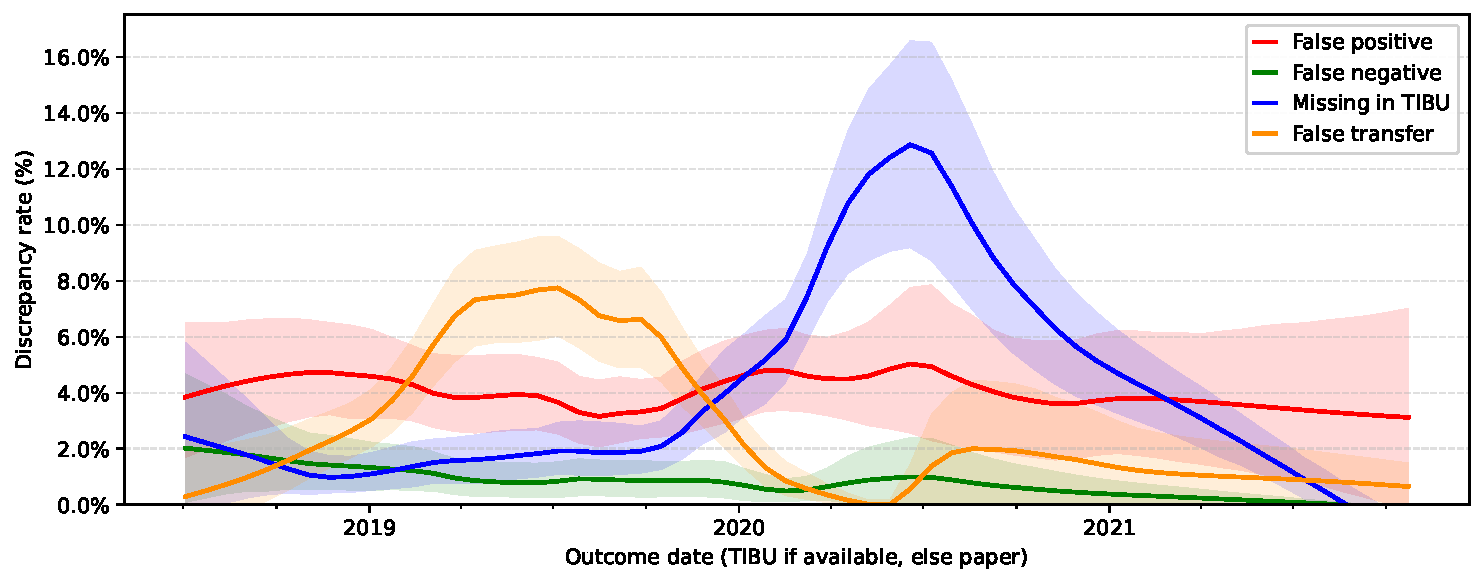
\includegraphics[width=0.85\textwidth]{fig_error_over_time.pdf}
    \caption{DQA error rates over time.}
    \label{fig:over_time}
\end{figure}

\end{document}
